\documentclass[%
%reprint,
%superscriptaddress,
%groupedaddress,
%unsortedaddress,
%runinaddress,
%frontmatterverbose, 
%preprint,
%preprintnumbers,
nofootinbib,
% longbibliography,
%nobibnotes,
%bibnotes,
 amsmath,amssymb,
 aps,
 prd,
%pra,
%prb,
%rmp,
%prstab,
%prstper,
%floatfix,
%twocolumn
10pt]{revtex4-2}

% \usepackage[inline]{showlabels}

\usepackage{graphicx}
\usepackage{braket}
\usepackage{hyperref}
\usepackage{bm}
\usepackage{textcase}
\usepackage{mathrsfs}
\usepackage{subcaption}
\usepackage{listings}
\usepackage{bbm} % for \mathbbm{1}
\usepackage[capitalise]{cleveref} % for multiple equations reference \cref{A,B,C}

\usepackage{xcolor}
\newcommand{\red}[1]{\textcolor{red}{#1}}
\newcommand{\blue}[1]{\textcolor{blue}{#1}}
\newcommand{\gray}[1]{\textcolor{gray}{#1}}
\newcommand{\brown}[1]{\textcolor{brown}{#1}}
\renewcommand{\d}{\ensuremath{\mathrm{d}}}
\newcommand{\M}{\mathcal{M}}
\newcommand{\A}{\mathcal{A}}
\renewcommand{\O}{\mathcal{O}}
\renewcommand{\Re}{\mathrm{Re}}
\renewcommand{\Im}{\mathrm{Im}}
\renewcommand{\dim}{\mathrm{dim}}
\newcommand{\End}{\mathrm{End}}
\newcommand{\R}{\mathbb{R}}
\newcommand{\Id}{\mathbbm{1}}
\newcommand{\Tr}{\mathrm{Tr}}
\newcommand{\Arg}{\mathrm{Arg}}
\newcommand{\sign}{\mathrm{sign}}
\newcommand{\adj}{\mathrm{adj}}

\renewcommand{\H}{\hat{H}} % Hamiltonian
\newcommand{\HH}{\mathcal{H}} % Hamiltonian
\newcommand{\K}{\hat{K}} % space shift generator
\newcommand{\h}{\bm h} % Hamiltonian vector
\newcommand{\hsub}{\kappa} % Hamiltonian vector
\newcommand{\hhsub}{\bm \kappa} % Hamiltonian vector


\newcommand{\llambda}{\bm{\lambda}} % Lie group generators
\newcommand{\coord}{\beta} %  general coordinate of the param. space
\newcommand{\ccoord}{\bm{\beta}}
\renewcommand{\c}{\mathcal C} %circumference
\newcommand{\PT}{\mathcal{PT}} %PT symmetry
\renewcommand{\path}{\gamma} %path in parameter space

%k is for energy levels, goes up to N = dim H
%i,j,k are indices
%greek is for geometrical stuff, mu,nu,xi are general indices marking direction in param. space

\usepackage{tcolorbox}
\tcbuselibrary{theorems}
\newtcbtheorem{fcitation}{Citation}{colback=gray!10, colframe=gray!70!blue}{def}

\begin{document}

\title{State driving of the Lipkin-Meshkov-Glick model on a quantum computer}
\date{\today}
\author{Jan Střeleček}
\maketitle



\section{Introduction}
\subsection{Model implementation}

We use reparametrization of an $N$ all-to-all interacting qubits model. Each qubit acts in its two-dimensional Hilbert space $\HH^{(i)}$, Lipkin-Meshkov-Glick (LMG)\cite{Cejnar23} as
\begin{equation}
   \H_{full} = -\frac{\lambda + 2\chi^2}{4} + \sum_i \left[\left(\frac{1}{2} - \frac{\chi^2}{2N}\right)\hat{\sigma}_z^{(i)} - \frac{\chi}{2N}\hat{\sigma}_x^{(i)}\right] - \frac{1}{4N}\sum_{i\neq j}\left[\lambda\hat{\sigma}_x^{(i)}\hat{\sigma}_x^{(j)} + \red{2}\chi\left(\hat{\sigma}_x^{(i)}\hat{\kappa}^{(j)} + \hat{\kappa}^{(i)}\hat{\sigma}_x^{(j)}\right) + \red{4}\chi^2\hat{\kappa}^{(i)}\hat{\kappa}^{(j)}\right]
   \label{eq:hamiltonian_full}
\end{equation}
for $\kappa^{(i)}\equiv \frac{1+\sigma_z^{(i)}}{2}$. \red{These factors seem to be wrong in the article, I got them from our $J_i$ Lipkin below and numerically it fits. In my thesis, I got it probably correct with the red fix above.}

This model lives in rather large space $\H_{full}\in\End( \HH_{full})$ with $\dim \HH_{full}=2^N$. Since the collective spin operator $\hat J$ commutes $[\H_{full},\hat J^2]=0$, we can restrict the system to some $j$-preserving subspace, for which we choose the maximal spin $j=N/2$. In this Hilbert subspace, one can rewrite the Hamiltonian as\cite{Strelecek25}
\begin{equation}
    \H = J_z - \frac{1}{N}\left\{\lambda J_x^2 + \chi\left[J_x\left(J_z + \frac{N}{2}\right) + \left(J_x + \frac{N}{2}\right)J_z\right] + \chi^2\left(J_z + \frac{N}{2}\right)^2\right\}.
    \label{eq:hamiltonian_j_max}
\end{equation}
This system acts in $\H\in\End(\HH)$ with $\dim\HH=N+1$. This is much smaller space and we will assume the $j=N/2$ restriction from now on.

To implement this model on a quantum computer, one needs to rewrite the model back into Pauli $\sigma$-matrix representation. This can be done directly from the matrix representation of our Hamiltonian \ref{eq:hamiltonian_j_max} in Spherical harmonics basis $\ket{j,m}$ for quantum numbers $j$ as the angular momentum and $m$ its projection to the direction of $\hat J_3
$. This results in penta-diagonal matrix, which 
needs to be embedded in the Hilbert space generated by $N_\mathrm q=\lceil \log_2(\dim \H)\rceil = \lceil \log_2(N+1)\rceil$ qubits, which has dimension $2^{N_\mathrm d}$. For example, $N=5$ Hamiltonian requires $3$ qubit Hilbert space
\begin{equation}
\H^{(N=5)} = \begin{pmatrix}
\blue{\bullet} & \blue{\bullet} & \blue{\bullet} & 0 & 0 & 0 & \gray{0} & \gray{0} \\
\blue{\bullet} & \blue{\bullet} & \blue{\bullet} & \blue{\bullet} & 0 & 0 & \gray{0} & \gray{0} \\
\blue{\bullet} & \blue{\bullet} & \blue{\bullet} & \blue{\bullet} & \blue{\bullet} & 0 & \gray{0} & \gray{0} \\
0 & \blue{\bullet} & \blue{\bullet} & \blue{\bullet} & \blue{\bullet} & \blue{\bullet} & \gray{0} & \gray{0} \\
0 & 0 & \blue{\bullet} & \blue{\bullet} & \blue{\bullet} & \blue{\bullet} & \gray{0} & \gray{0} \\
0 & 0 & 0 & \blue{\bullet} & \blue{\bullet} & \blue{\bullet} & \gray{0} & \gray{0} \\
\gray{0} & \gray{0} & \gray{0} & \gray{0} & \gray{0} & \gray{0} & \gray{0} & \gray{0} \\
\gray{0} & \gray{0} & \gray{0} & \gray{0} & \gray{0} & \gray{0} & \gray{0} & \gray{0}
\end{pmatrix}
\label{eq:Binary_Hamiltonian_embedding}
\end{equation}
One could even offset the diagonal elements of the extra space to some large energies, to be physically consistent with spectrum ordering, creating the Hamiltonian $\H\otimes \zeta \Id_{2^{N_\mathrm d}-(N-1)}$ for some $\zeta\gg E_N$. Such a Hamiltonian can be rewritten using Qiskit \texttt{SparsePauliOp.from\_operator()}\footnote{\url{https://quantum.cloud.ibm.com/docs/en/api/qiskit/qiskit.quantum_info.SparsePauliOp}} function into Hamiltonian acting on 3 qubits 
\begin{equation}
    \H_{3q}=\alpha_1 \hat I\hat I\hat I + \alpha_2 \hat I\hat I\hat X + \alpha_3 \hat I\hat I\hat Z + \dots \alpha_k \hat Z \hat Z \hat Z,
\end{equation}
where operators are tensor multiplied and their order marks qubit on which they act.

This is called \emph{Binary encoding} or \emph{computational basis encoding} and it requires few qubits, but the circuit depth can be rather large when implementing quantum state driving. We will try to make a trade "depth for qubits" by using another encoding.


\subsubsection{One-hot encoding}
The name of \emph{one-hot encoding} (sometimes called \emph{Unary encoding}) comes from the premise that we want only one qubit hot (in state $\ket{1}$) and others in state $\ket{0}$. The Hamiltonian \ref{eq:hamiltonian_j_max} requires $N+1$ qubits (which is more than in Binary encoding), but the circuit depth should decrease substantially. This is because number of Pauli terms required to implement the Hamiltonian decreases to $3N+1$. In comparison, optimal encoding for the number of qubits would probably be Gray code encoded Hamiltonian \ref{eq:hamiltonian_j_max} requiring $N_\mathrm q = \lceil \log_2(N+1)\rceil$ qubits to implement the Hamiltonian, which itself would require $2^{N_\mathrm q}+N_\mathrm q 2^{N_\mathrm q-1}-1$ Pauli terms \cite{Matteo21}.

\begin{fcitation}{\cite{Matteo21}}
{}\centering
\begin{tabular}{lcc}
\hline\hline
& \textbf{One-hot} & \textbf{Gray code} \\
\hline
Qubits & $N$ & $\lceil \log_2 N \rceil = \eta$ \\
Number of Pauli terms & $3N-2$ & $2^\eta + \eta 2^{\eta-1} - 1$ \\
Commuting sets of Paulis & 3 & $\eta + 1$ \\
Max Pauli weight & 2 & $\eta$ \\
\hline\hline
\end{tabular}
\end{fcitation}

To implement the model, we first map the basis and show how to implement the Hamiltonian and some state vector. In the section \ref{sec:time_evolution} we show how the time evolution simplifies in this representation.

\textbf{Basis mapping}

The Hamiltonian \ref{eq:hamiltonian_j_max} acts in $(N+1)$-dimensional Hilbert space spanned by states $\{\ket{j,m}\}$ for $j=N/2$ and $m \in \{-N/2, -N/2+1, \ldots, N/2\}$. In one-hot encoding \cite{Sawaya20,Matteo21}, we map each physical state to a computational basis state with $N+1$ qubits:
\begin{equation}
    \ket{j,m_i} \longrightarrow \ket{0\cdots 0 \overset{i}{1} 0 \cdots 0};\qquad i=1,\dots,N.
\end{equation}
Under this encoding, the $i$-th state (as in the $\ket{j,m}$ basis) is mapped to the $i$-th qubit as
\begin{align*}
    \ket{j,-j} &\mapsto \ket{10\dots 0}\\
    &\;\;\vdots\\
    \ket{j,j} &\mapsto \ket{0\dots 01}
\end{align*}

\textbf{Hamiltonian mapping}

The Hamiltonian \ref{eq:hamiltonian_j_max} in the $\{\ket{j,m}\}$ basis is represented as $(N+1) \times (N+1)$ penta-diagonal matrix:
\begin{equation}
    \H = \begin{pmatrix}
        h_0 & c_0 & d_0 & 0 & \cdots \\
        c_0 & h_1 & c_1 & d_1 & \cdots \\
        d_0 & c_1 & h_2 & c_2 & \ddots \\
        0 & d_1 & c_2 & \ddots & \ddots \\
        \vdots & \vdots & \ddots & \ddots & \ddots
    \end{pmatrix}
\end{equation}
where $h_i = \bra{i}\H\ket{i}$ are diagonal energies, $c_i = \bra{i+1}\H\ket{i}$ are nearest-neighbor (NN) couplings, and $d_i = \bra{i+2}\H\ket{i}$ are next-nearest-neighbor (NNN) couplings.

To implement on a quantum computer, we rewrite the Hamiltonian using Pauli operators. We construct projection operators acting on $n$th qubit
\begin{equation}
    P_0^{(n)} = \frac{1}{2}(\Id + \hat{\sigma}_z^{(n)}) = \ket{0}\bra{0}; \quad P_1^{(n)} = \frac{1}{2}(\Id - \hat{\sigma}_z^{(n)}) = \ket{1}\bra{1}
\end{equation}

Ladder-type operators in one-hot encoding transform states such that in positions $n$ and $n+1$ we get from $\ket{10}$ to $\ket{01}$. This can be implemented as
\begin{equation}
    \frac{1}{2}(\hat{\sigma}_x^{(n)}\hat{\sigma}_x^{(n+1)} + \hat{\sigma}_y^{(n)}\hat{\sigma}_y^{(n+1)}) \ket{0...\overset{n}{1}0...0}=  \ket{0...0\overset{n+1}{1}...0}
\end{equation}

The complete penta-diagonal Hamiltonian in one-hot encoding becomes:
\begin{equation}
\begin{split}
    \H &=\overbrace{\sum h_n \ket{n}\bra{n}}^{H_{\mathrm{diag}}} + \overbrace{\sum c_n \left(\ket{n}\bra{n+1}+\text{h.c.}\right)}^{H_{\mathrm{NN}}} + \overbrace{\sum d_n \left( \ket{n}\bra{n+2}+\text{h.c.}\right)}^{H_{\mathrm{NNN}}} \\
    &= \frac{1}{2}\sum_{n=0}^{N} h_n (\Id - \hat{\sigma}_z^{(n)}) + \frac{1}{2}\sum_{n=0}^{N-1} c_n (\hat{\sigma}_x^{(n)}\hat{\sigma}_x^{(n+1)} + \hat{\sigma}_y^{(n)}\hat{\sigma}_y^{(n+1)}) + \frac{1}{2}\sum_{n=0}^{N-2} c_n (\hat{\sigma}_x^{(n)}\hat{\sigma}_x^{(n+2)} + \hat{\sigma}_y^{(n)}\hat{\sigma}_y^{(n+2)})
\end{split}
\end{equation}  

This requires only $\O(N)$ Pauli terms, significantly fewer than binary encoding which requires $\O(2^n)$ terms for $n = \lceil \log_2(N+1) \rceil$ qubits\cite{Matteo21}.



\textbf{State preparation}

The ground state $\ket{\psi_0} = \sum_{i=0}^{N} c_i \ket{i}$ can be prepared using a cascade of controlled rotations:
\begin{equation}
    \ket{100\cdots0} \xrightarrow{\text{CRY}(\theta)} \alpha_0\ket{100\cdots} + \beta_0\ket{110\cdots} \xrightarrow{\text{CX(1,0)}} \alpha_0\ket{100\cdots} + \beta_0\ket{010\cdots} \xrightarrow{\text{CRY+CX}} \cdots \Rightarrow \sum_{i=0}^{N} c_i \ket{i},
\end{equation}
which has circuit depth $\O(N)$. This can be shortened to $\O(\log^2 N)$ \cite{Chen24}, but since this is not the caveat of complexity in quantum state driving we stick to the simple implementation here.





\subsection{Discretization of the time evolution}
\label{sec:time_evolution}
The necessity of discretizing the continuous Hamiltonian evolution into a set of unitary gates is a disadvantage of gate-based quantum computing over quantum annealing. Trotterization is one method for this discretization of a system. The Hamiltonian $\hat H(\lambda)$ with a real parameter $\lambda$, time evolution $\hat U$ has to be discretized to its digitized approximation on $M$ unitary gates $\hat U_d^{(M)}$. When asking for a complexity of such decomposition, one asks for conditions under which some initial state $\ket{\psi_0}$ can be evolved into approximately correct final state, i.e. $||(\hat U-\hat U_d^{(M)}\ket{\psi_0}|| \leq \epsilon$ for some evolution error $\epsilon$. The complexity scaling then means \emph{to get error $\epsilon$, one needs $M= \O($\textit{some function of driving time, minimal energy gap along the driving protocol, ...}}) \emph{gates}.

The resulting circuit depth will depend on the initial Hamiltonian complexity, which differs a lot between binary and one-hot encoding.

Performing the time evolution using time dependent Hamiltonian $\H(t)$ increases the complexity $T/\d t$ times, where $T$ is the final driving time and $\d t$ is the time segment, since the transformation of the evolution operator $\hat U(t+\d t|t)$ from time $t$ by step $\d t$ requires the Hamiltonian to be constant.
Implementing $\hat U(t+\d t|t)$ by Trotterizing $\H(t=fixed)$ which is binary encoded can be done in Qiskit using \texttt{PauliEvolutionGate(H, time=dt, synthesis=SuzukiTrotter(order=p))} \emph{Suzuki Trotter decomposition} of order $p$. Such a step requires $2L 5^{p-1}$ exponentials for $L$ the number of unitaries in the Hamiltonian $\H=\sum_{i=1}^L \H_i$ \cite{Wiebe10}.


For one-hot encoding, we can write our own time step evolution with smaller depth.

\textbf{Time evolution via Trotterization}

Suzuki-Trotter decomposition of first order for operators $\hat A$, $\hat B$ gives \cite{Hatano05}
\begin{align*}
    \text{First order: }&e^{\delta (A+B)}= e^{\delta A}e^{\delta B}+\O(\delta^2) \\
    \text{Second order: }&e^{\delta (A+B)}= e^{\delta B/2}e^{\delta A}e^{\delta B/2}+\O(\delta^3)
\end{align*} 
For time evolution $e^{-i\H \Delta t}$ we get
\begin{align}
    \text{First order: } e^{-i\H \Delta t} &= e^{-i\H_{\mathrm{diag}} \Delta t} e^{-i\H_{\mathrm{NN}} \Delta t} e^{-i\H_{\mathrm{NNN}} \Delta t} + \O(\Delta t^2)\\
     \text{Second order: }e^{-i\H \Delta t} &= e^{-i\H_{\mathrm{diag}} \frac{\Delta t}{2}} e^{-i\H_{\mathrm{NN}} \frac{\Delta t}{2}} e^{-i\H_{\mathrm{NNN}} \Delta t} e^{-i\H_{\mathrm{NN}} \frac{\Delta t}{2}} e^{-i\H_{\mathrm{diag}} \frac{\Delta t}{2}} + \O(\Delta t^3)
\end{align}


\textit{Diagonal terms:} From $\frac{h_n}{2}(\Id - \hat{\sigma}_z^{(n)})$, time evolution gives:
\begin{equation}
    e^{-i\frac{h_n}{2}(\Id - \hat{\sigma}_z^{(n)})\Delta t} = e^{-i\frac{h_n \Delta t}{2}}  e^{i\frac{h_n \Delta t}{2}\hat{\sigma}_z^{(n)}} = e^{-i\frac{h_n \Delta t}{2}}RZ(-h_n \Delta t, n)
\end{equation}
The global phase $e^{-i\frac{h_n \Delta t}{2}}$ can be omitted as a gauge choice.

\textit{Off-diagonal terms:} From $\frac{c_n}{2}(\hat{\sigma}_x^{(n)}\hat{\sigma}_x^{(n+1)} + \hat{\sigma}_y^{(n)}\hat{\sigma}_y^{(n+1)})$:
\begin{equation}
    R_{XY}^{(n,m)}(c_n \Delta t) = e^{-i\frac{c_n}{2}(\hat{\sigma}_x^{(n)}\hat{\sigma}_x^{(m)} + \hat{\sigma}_y^{(n)}\hat{\sigma}_y^{(m)})\Delta t},
\end{equation}
which is the XY gate\footnote{\url{https://quantum.cloud.ibm.com/docs/en/api/qiskit/qiskit.circuit.library.XXPlusYYGate}}, which naturally implements the hopping $\ket{10} \leftrightarrow \ket{01}$ in the one-hot subspace. Qiskit's \texttt{XXPlusYYGate} provides an efficient 2-CNOT decomposition.

\textbf{Final evolution step}

Putting all together, we get the unitary evolution for a time step $\Delta t$. Defining the hopping gate acting on qubits $n, m$ with strength $k$ as , the first-order Trotter step is:

\begin{equation}
    \begin{aligned}
    \hat U(t+\Delta t, t) \approx \;& \Bigg[\prod_{n=0}^{N} R_Z^{(n)}(-h_n \Delta t) \Bigg] \\
    &\cdot \Bigg[ \prod_{k \in S_{\text{odd}}^{(1)}} R_{XY}^{(k, k+1)}(c_{k} \Delta t) \Bigg] \cdot \Bigg[ \prod_{k \in S_{\text{even}}^{(1)}} R_{XY}^{(k, k+1)}(c_{k} \Delta t) \Bigg] \\
    &\cdot \Bigg[ \prod_{k \in S_{A}^{(2)}} R_{XY}^{(k, k+2)}(d_{k} \Delta t) \Bigg] \cdot \Bigg[ \prod_{k \in S_{B}^{(2)}} R_{XY}^{(k, k+2)}(d_{k} \Delta t) \Bigg]
    \end{aligned}
\end{equation}
where the nearest-neighbor sets are standard odd/even $S_{\text{odd}}^{(1)} = \{1, 3, \dots\}$, $S_{\text{even}}^{(1)} = \{0, 2, \dots\}$. 
The next-nearest-neighbor sets must avoid range-2 collisions (e.g., $0-2$ colliding with $2-4$), so we define:
$S_{A}^{(2)} = \{k \mid k \pmod 4 \in \{0, 1\}\}$ and $S_{B}^{(2)} = \{k \mid k \pmod 4 \in \{2, 3\}\}$.

\subsection{Transpilation}
For the transpilation, we can set
\begin{itemize}
    \item optimization level for transpilation\footnote{\url{https://quantum.cloud.ibm.com/docs/en/guides/set-optimization}} on QC,\texttt{optimization\_level = 3}, for which operations trying to simplify and nest the sequences single and two-qubit gates are applied,
    \item layout method\footnote{\url{https://quantum.cloud.ibm.com/docs/en/api/qiskit/qiskit.transpiler.Layout}}:  \texttt{layout\_method='sabre'} and \texttt{routing\_method='sabre'} which defines how virtual qubits are mapped to physical\footnote{\url{https://quantum.cloud.ibm.com/docs/en/api/qiskit/transpiler\#transpiler-preset-stage-layout}}, 
    \item \texttt{translation\_method='default'} defines how to rewrite circuit to quantum computer native gates\footnote{\url{https://quantum.cloud.ibm.com/docs/en/api/qiskit/transpiler\#transpiler-preset-stage-translation}},
    \item \texttt{approximation\_degree = 1.} sets how precisely the implemented circuit matches the desired one. This can substantially reduce the number of gates, while increasing the error \footnote{\url{https://qiskit.qotlabs.org/docs/guides/common-parameters}}.
\end{itemize}

\subsection{Measurement}
We use \texttt{Estimator} to measure the while wavefunction. We also obtain the eigenvectors of Hamiltonian $\H(T)$ classically to convert the result into the final time eigenbasis. This is cheating and in reality should be done on quantum computer (since it is a hard task), but since real experiment would not care about the eigenbasis or would measure some observable (like magnetization), we will not care about this. 

\section{Driving example}
The state at time $t=0$ is initialized as a ground state of $\H(0)$. This computation is performed classically, which is sort of "cheating", since it is hard task and should in reality be performed on quantum computer. For practical applications the state is usually prepared in some easy to prepare state (that is the point of driving), such as $\ket{0\dots 0}$. Also we want to focus on the time evolution part in this experiment.

As an example, we chose LMG from Eq. \ref{eq:hamiltonian_j_max} with $N=5$ and driving path which linearly interpolates between points in parameter space of $\H(\lambda,\chi)$
\begin{equation}
    \begin{split}
    (\lambda_0,\chi_0 )&= (-0.5,0)\\
    (\lambda_T,\chi_T )&= (-0.3,1.5)
    \label{eq:driving_path}
    \end{split}
\end{equation}
This path is shown in Fig. \ref{fig:driving_path_N=5} along with QPT (arrising in he infinite size limit of LMG) and diabolic points. The Hamitlonian spectrum is shown in Fig. \ref{fig:driving_path_N=5_spectrum}.

\begin{figure}[h]
    \centering
    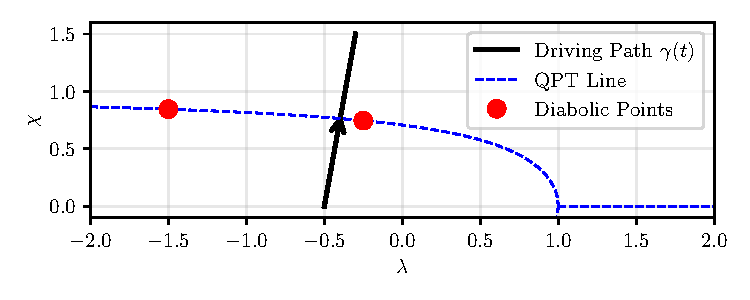
\includegraphics{img/driving_path_N=5.pdf}
    \caption{Driving path defined in Eq. \eqref{eq:driving_path} with QPT and diabolic points for LMG $N=5$ model. The arrow shows the direction of driving.}
    \label{fig:driving_path_N=5}
\end{figure}
\begin{figure}[h]
    \centering
    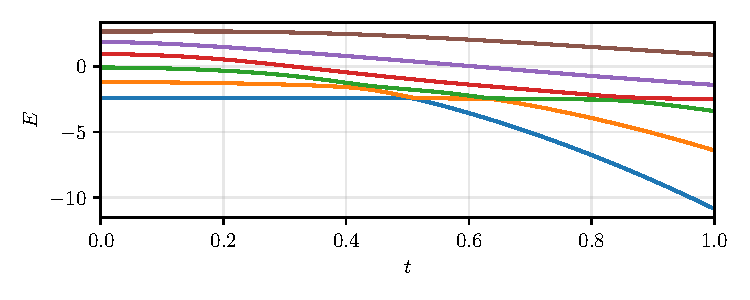
\includegraphics{img/driving_path_N=5_spectrum.pdf}
    \caption{Spectrum along driving path in Eq. \eqref{eq:driving_path} for LMG $N=5$ model.}
    \label{fig:driving_path_N=5_spectrum}
\end{figure}

\subsection{Binary encoding}
The dimension of the Hilbert space is $N+1=6$, which needs to be embedded in $8-$dim Hilbert space spanning over 3 qubits as shown in Eq. \eqref{eq:Binary_Hamiltonian_embedding}. The extra levels will be offset by $10^{10}$ (and ignored in the spectrum above). The Hamiltonian at initial position, decomposed into sum of unitaries (again ignoring the extra levels), visualized in Fig. \ref{fig:midTime_Hamiltonian_N=5}. Note there are 24 elements (smaller than $10^9$) and 4 larger than that, corresponding to unphysical levels.


\begin{figure}[h!]
    \centering
    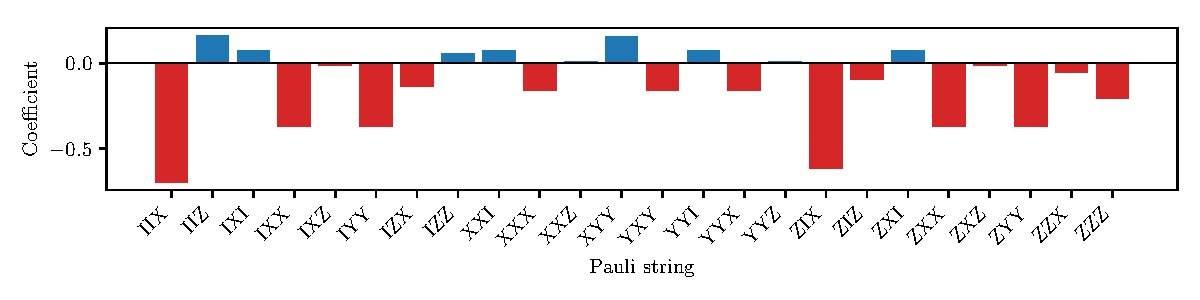
\includegraphics[width=\textwidth]{img/midTime_Hamiltonian_N=5.pdf}
    \caption{Coefficients of Pauli decomposition of Hamiltonian $\H(t=0.5 T)$ for LMG $N=5$ model in binary encoding.}
    \label{fig:midTime_Hamiltonian_N=5}
\end{figure}

If the time evolution consisted of only a single large time step ($n=1$, the first order Trotter would lead to around 119 gates with circuit depth 90, see Fig. \ref{fig:gates_single_step_evolution}. The second order Trotter would lead to around 173 gates with circuit depth 129.

\begin{figure}[h]
    \centering
    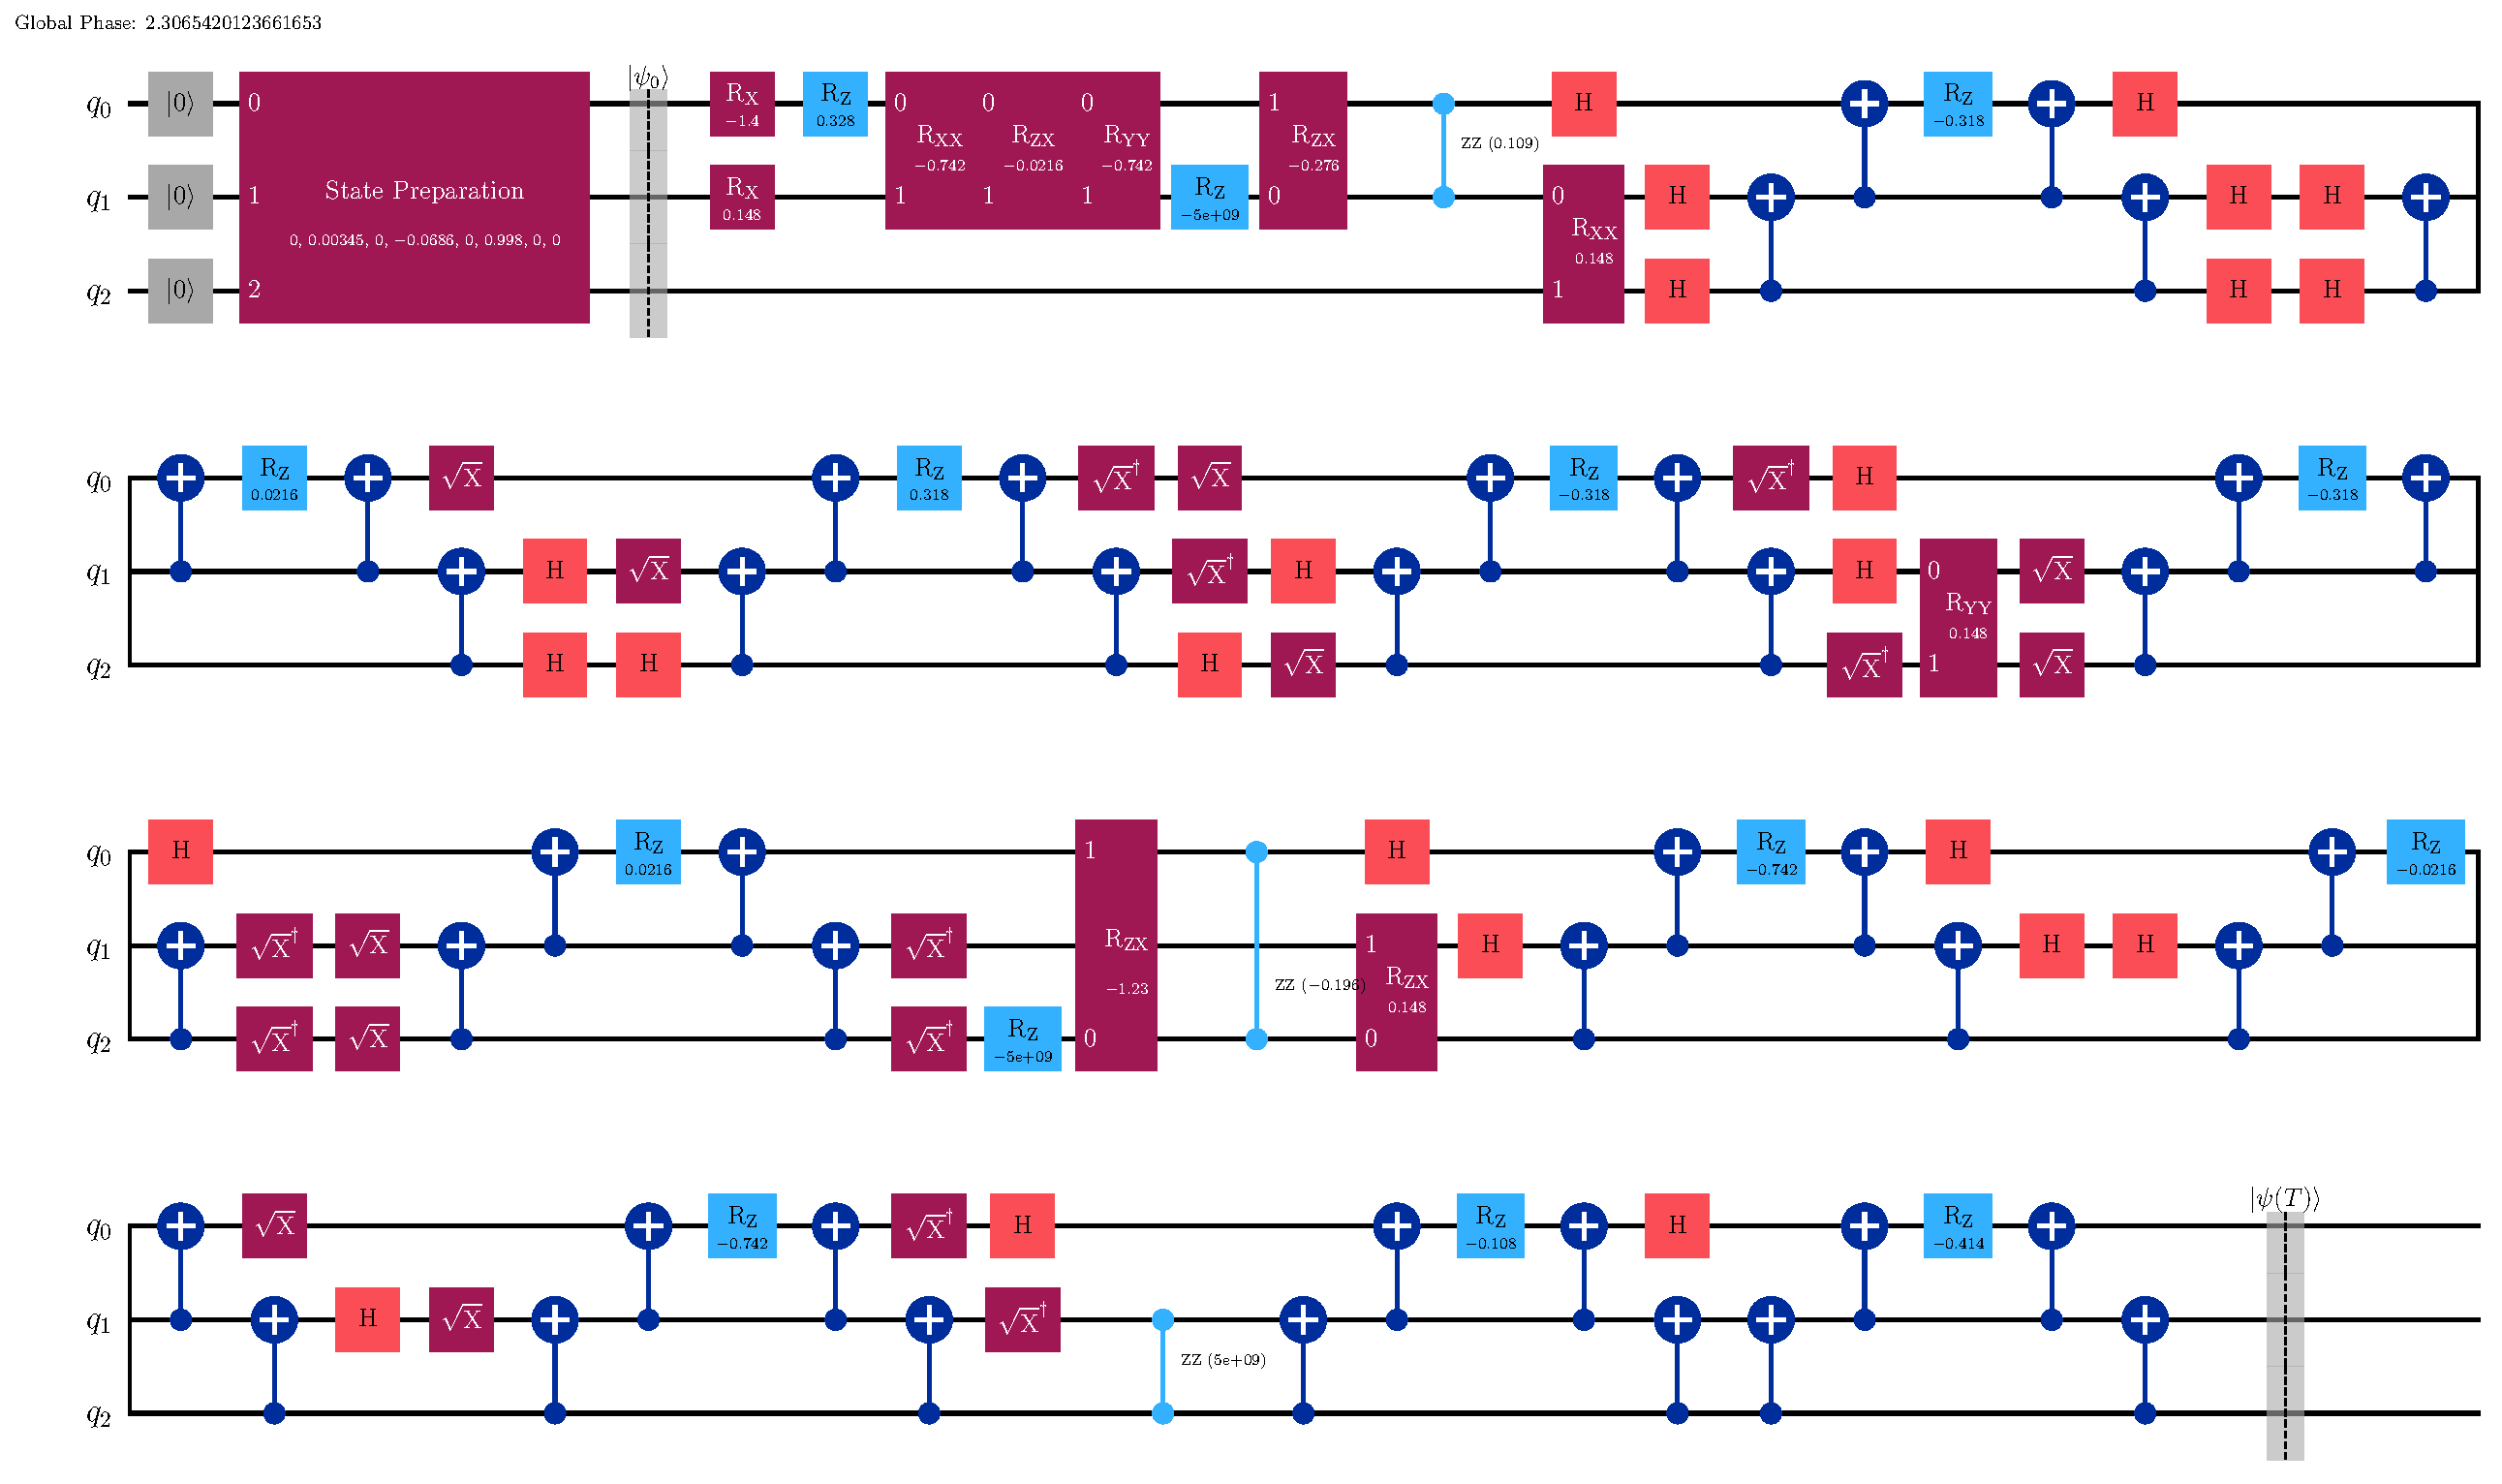
\includegraphics[width=\textwidth]{img/gates_single_step_evolution_N=5.pdf}
    \caption{Quantum circuit for single step time evolution of LMG $N=5$ model in binary encoding with first order Trotterization. This corresponds to evolution by $\H(t=0.5 T)$.}
    \label{fig:gates_single_step_evolution}
\end{figure}
Now we can attempt to approximate the quantum state driving. We compare 4 results:
\begin{itemize}
    \item \textbf{Exact}: Classical simulation of continuous time evolution. This represents the exact solution up to small numerical error caused by integration. The implementation uses \texttt{scipy.solve\_ivp()} with the \texttt{RK45} adaptive Runge-Kutta method, employing relative tolerance $10^{-10}$ and absolute tolerance $10^{-12}$.    
    \item \textbf{Exact discretized}: Classical piecewise-constant simulation that mirrors the time discretization used in quantum simulation, but without Trotter decomposition which leads to additional errors. Each time step applies the exact unitary $U(t+\d t|t)=e^{-i H(t+\d t/2)\d t}$ computed via matrix exponentiation (\texttt{scipy.linalg.expm}), where the Hamiltonian is evaluated at the midpoint of each interval. This method uses the same timestep $\d t = T/n_{\mathrm s}$ as the Trotterized quantum circuit. This method shows what is the error purely from time discretization.
    \item \textbf{Noiseless quantum simulator}: The Qiskit \texttt{AerSimulator} with \texttt{statevector} method, which classically executes the transpiled circuit that would run on hardware, including any approximations introduced during synthesis (controlled by \texttt{approximation\_degree}). The \texttt{EstimatorV2} primitive is used to compute expectation values of energy eigenstate projectors $\ket{E_k}\bra{E_k}$ (estimated from 4000 shots). This method adds errors from \emph{time discretization} of \emph{Trotter decomposition} (we use order 2) and \emph{gate synthesis errors}, but is still assuming ideal quantumn computer without noise.
    
    \item \textbf{Noisy quantum simulator}: The \texttt{AerSimulator.from\_backend()} method creates a simulator that incorporates the device-specific noise model extracted from the target IBM Quantum backend (e.g., \texttt{ibm\_aachen}). This includes single-qubit and two-qubit gate errors, readout errors, and decoherence characterized by $T_1$ (energy decay) and $T_2$ (dephasing) times. This simulation predicts the expected hardware behavior.
    \item \textbf{IBM Quantum computer}: The Trotterized time evolution circuit executed on real quantum hardware via the \texttt{EstimatorV2} primitive from \texttt{qiskit\_ibm\_runtime}. The circuit is transpiled using \texttt{preset\_pass\_manager} with configurable optimization level, layout, and routing strategies. Error mitigation techniques are applied including Twirled Readout Error eXtinction (TREX) and Zero-Noise Extrapolation (ZNE) at resilience level 2, with optional dynamical decoupling and Pauli twirling. Energy eigenstate populations are measured via expectation values of projector observables at final time $T$ ($|\braket{E_k|\psi}|^2$), which are obtained by classical exact diagonalization, which are clipped to $[0,1]$ and renormalized to account for small negative values arising from statistical fluctuations and imperfect error mitigation. This method can be more precise than noisy simulation since \emph{error mitigation} is applied.
\end{itemize}
The result of the run is shown in Fig. \ref{fig:final_comparison_binary}. The final infidelity 
\begin{equation}
    I = 1-|\braket{\psi_{\mathrm{exact}}|\psi_{\mathrm{final}}}|^2
\end{equation}
is calculated for each method as a measure of precition. It is shown in Fig. \ref{fig:driving_results_comparisong}.



\begin{figure}[h]
    \centering
    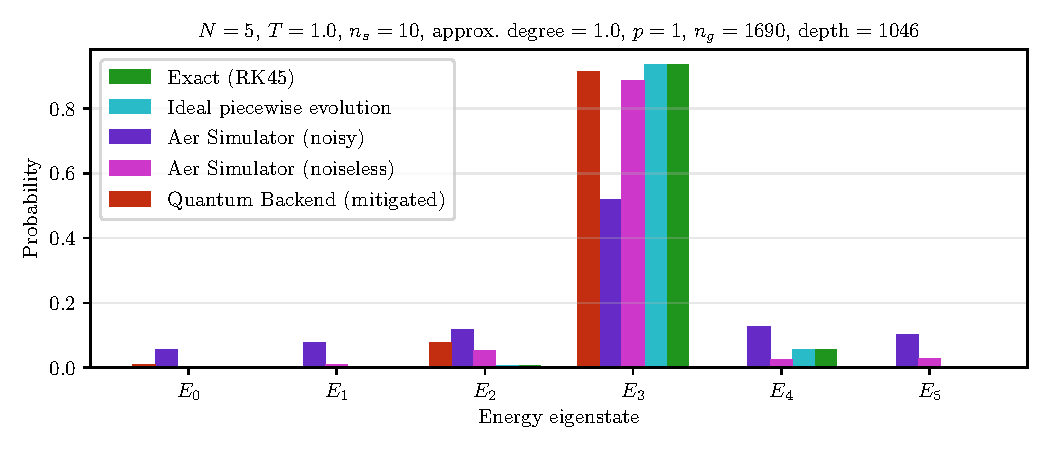
\includegraphics{img/final_comparison_binary.pdf}
    \caption{Quantum state driving of LMG $N=5$ model in binary encoding along path defined in Eq. \eqref{eq:driving_path}.}
    \label{fig:final_comparison_binary}
\end{figure}

\begin{figure}[h]
    \centering
    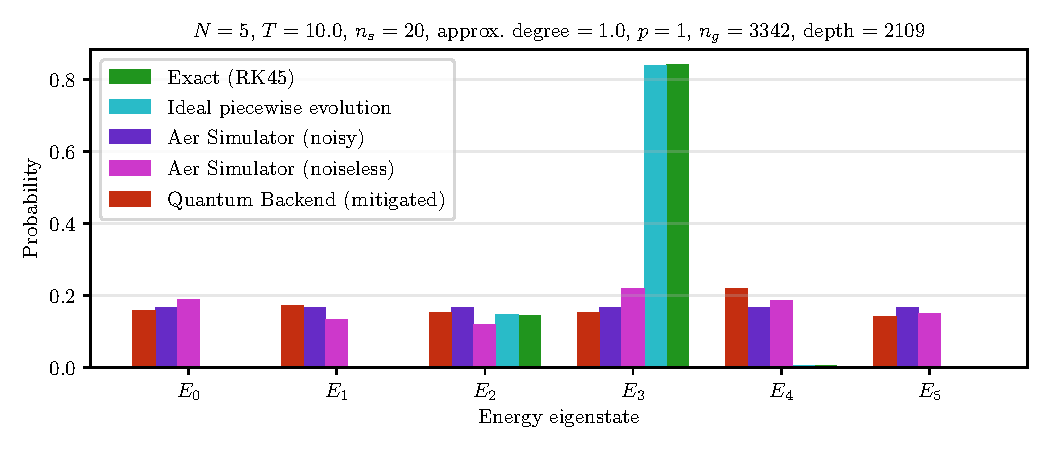
\includegraphics{img/final_comparison_binary_T=10.pdf}
    \caption{Quantum state driving of LMG $N=5$ model in binary encoding along path defined in Eq. \eqref{eq:driving_path} for longer driving time.}
    \label{fig:final_comparison_binary_T=10}
\end{figure}

\subsection{One-hot encoding}
In one-hot encoding, we treat diagonal, first neighbor and next-nearest neighbor terms separately. The Hamiltonian at mid-time is visualized in Fig. \ref{fig:lipkin_hamiltonian_N=5_midTime}. Diagonal elements are $h_n$, first neighbor couplings $c_n$ and next-nearest neighbor couplings $d_n$.

\begin{figure}[ht]
    \centering
    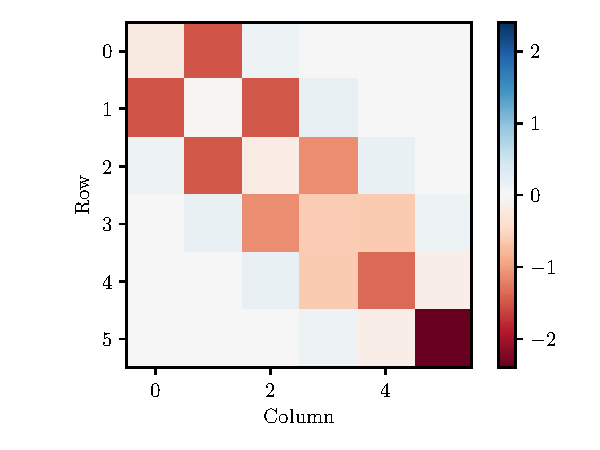
\includegraphics{img/lipkin_hamiltonian_N=5_midTime.pdf}
    \caption{Coefficients of Pauli decomposition of Hamiltonian $\H(t=0.5 T)$ for LMG $N=5$ model.}
    \label{fig:lipkin_hamiltonian_N=5_midTime}
\end{figure}

The unitary evolution step using mid-time Hamiltonian $\H(t=0.5 T)$ using first order Trotterization is shown in Fig. \ref{fig:gates_one_hot_single_step_evolution}. In comparison with binary encoding we get (excluding state preparation):
\begin{table}[ht]
\centering
\label{tab:circuit_comparison}
\begin{tabular}{lcccccc}
Encoding & Qubits & Gates & Depth & Transpiled gates & Transpiled depth  \\
\hline
Binary   & 3 & 115  & 88 & 232 & 137\\
One-hot  & 6 & 132  & 35 & 171 & 52 \\
\end{tabular}
\end{table}

\begin{figure}[h]
    \centering
    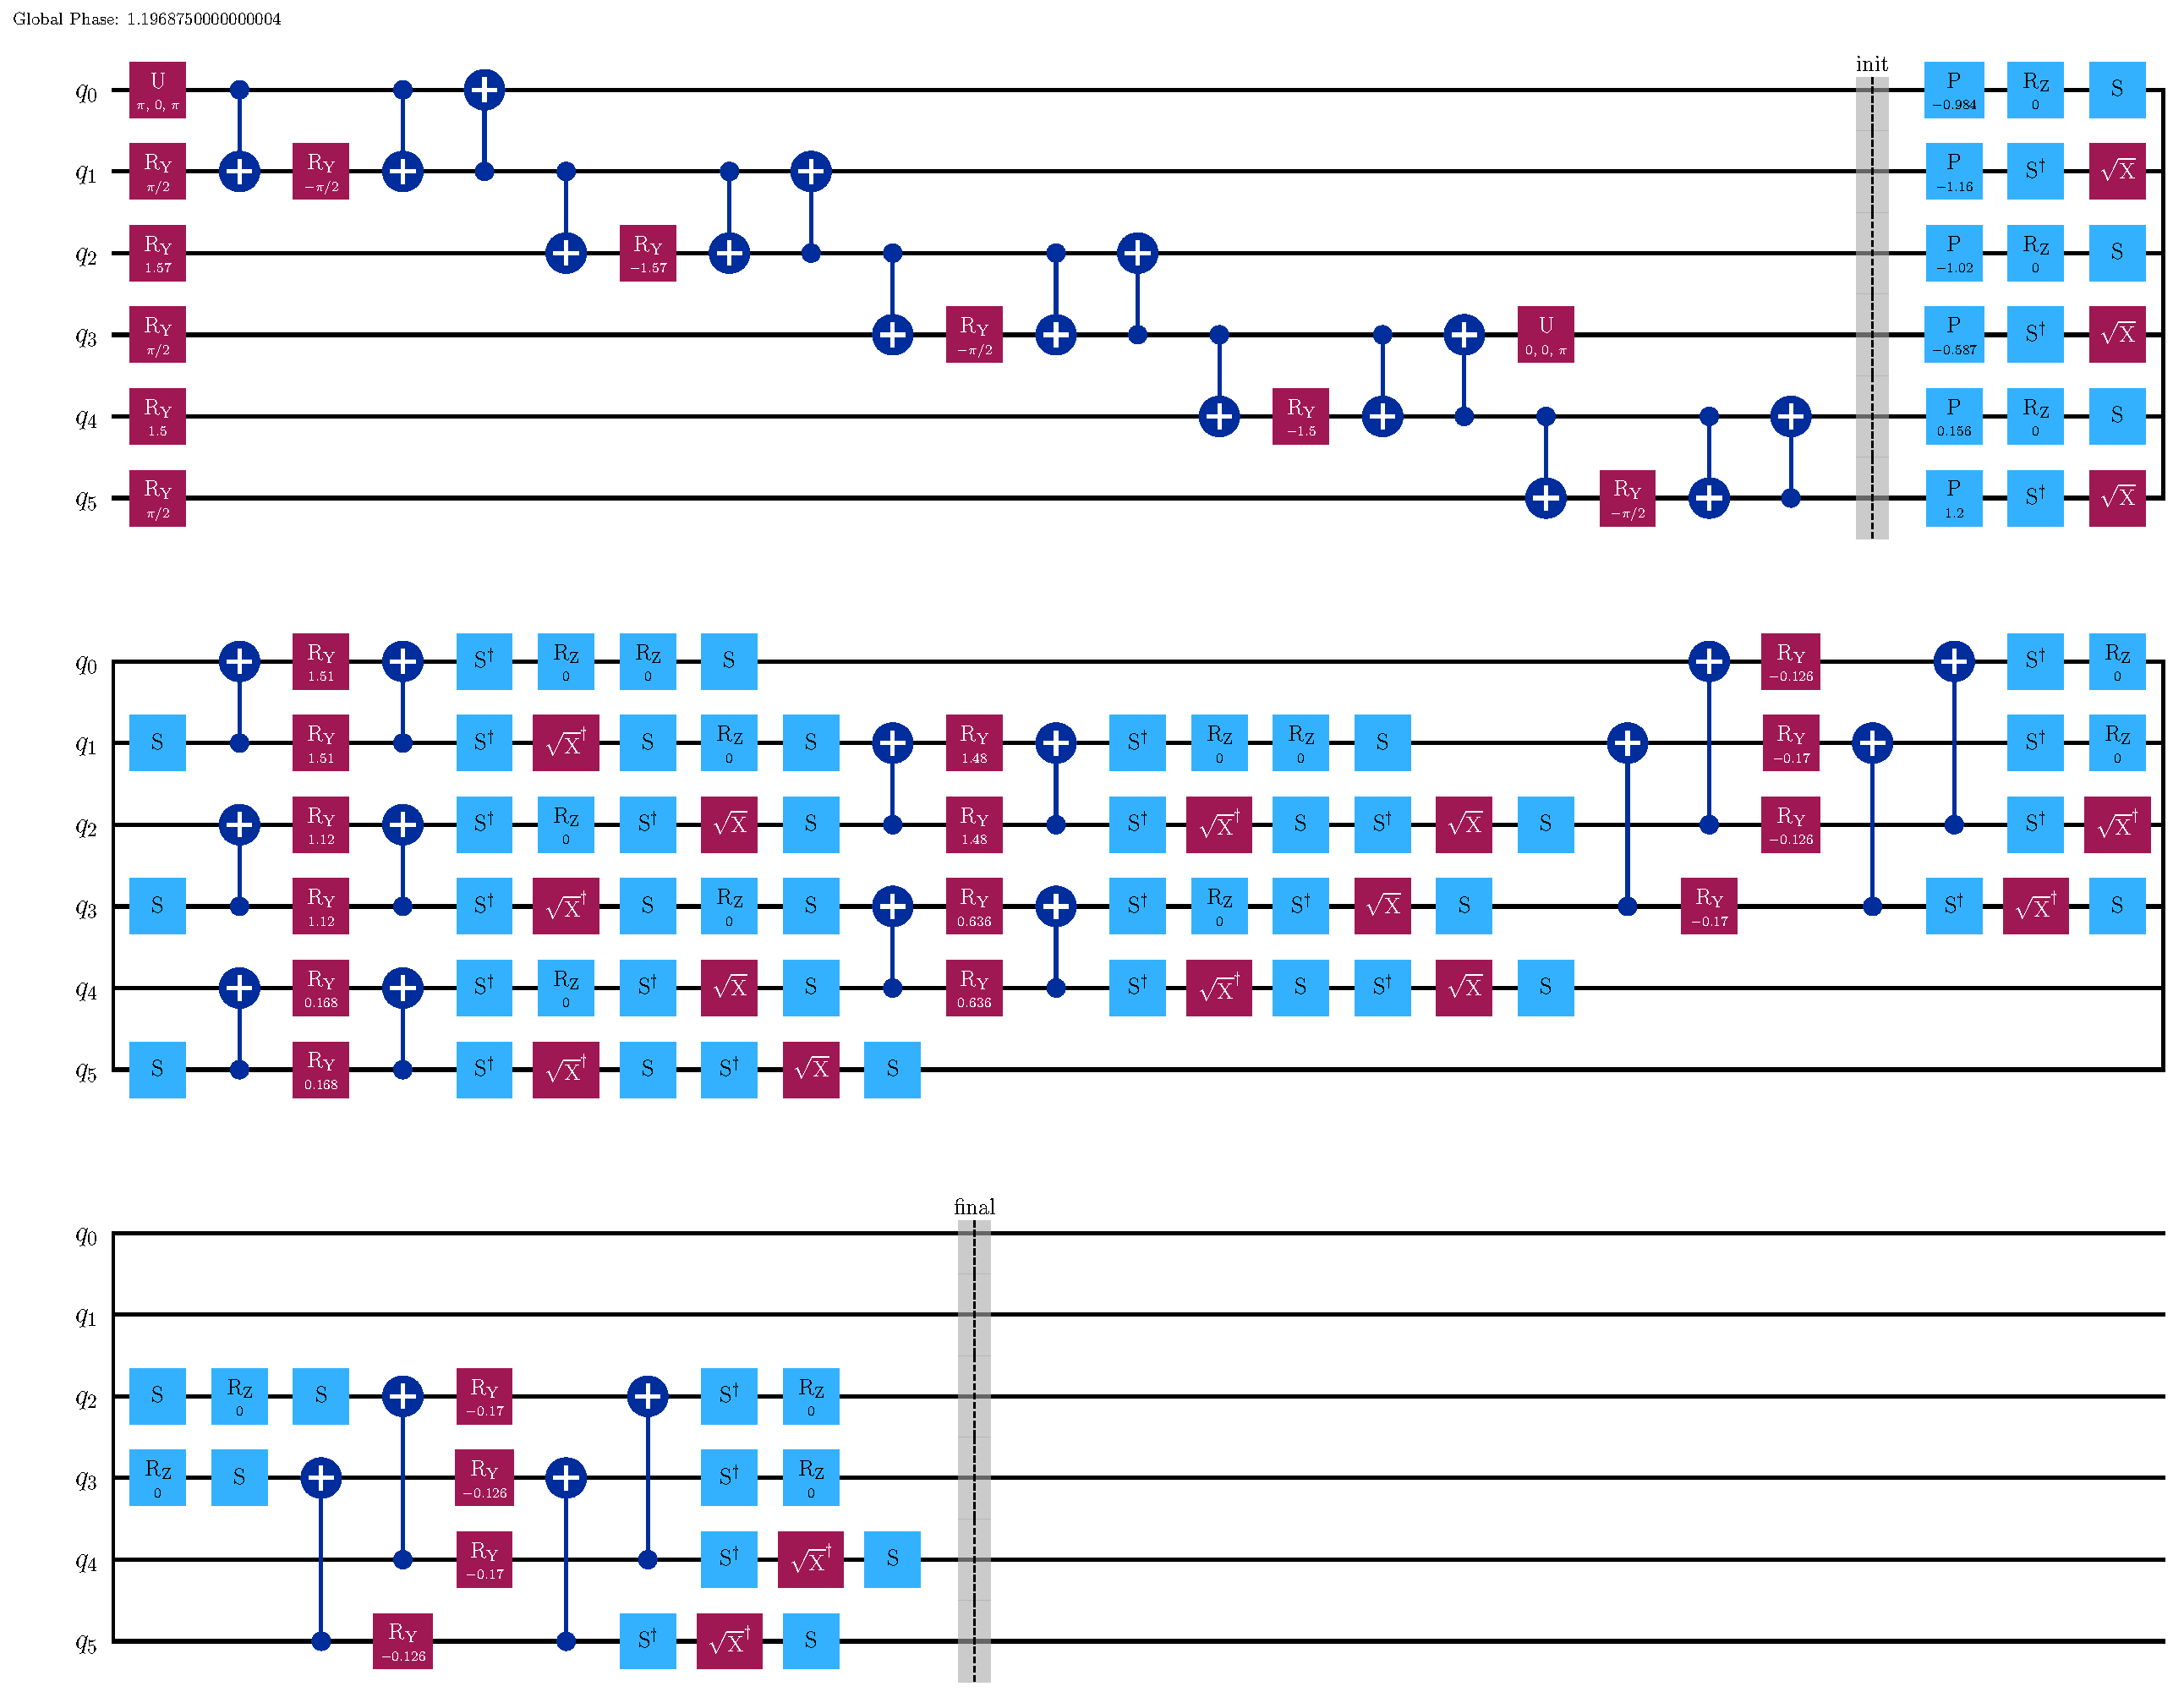
\includegraphics[width=\textwidth]{img/gates_one_hot_single_step_evolution_N=5.pdf}
    \caption{Quantum circuit for single step time evolution of LMG $N=5$ model in one-hot encoding with first order Trotterization. This corresponds to evolution by $\H(t=0.5 T)$.}
    \label{fig:gates_one_hot_single_step_evolution}
\end{figure}

The results are shown in Fig. \ref{fig:final_comparison_one_hot}. The final infidelity as compared to binary encoding is in Tab. \ref{tab:driving_results_comparisong}.
\begin{table}[h]
\centering
\begin{tabular}{l|cc|cc}
\textbf{Method} & \textbf{Infidelity (binary, A)} & \textbf{Infidelity (one-hot, A)} & \textbf{Infidelity (binary, secoBnd)} & \textbf{Infidelity (one-hot, B)} \\
\hline
Piecewise       & $2.8 \times 10^{-7}$  & $2.8 \times 10^{-7}$    & $1.5 \times 10^{-5}$ & $1.5 \times 10^{-5}$ \\
Aer (noiseless) & $0.0536$               & $0.00019$                & $0.58$              & $0.021$ \\
Aer (noisy)     & $0.315$                & $0.52$                   & $0.62$               & $0.26$ \\
Quantum Backend & $0.103$                & $0.55$                   & $0.65$               & $0.13$ \\
\end{tabular}
\caption{Comparison of infidelity between binary and one-hot and all used methods of computation. First (A) corresponds to $T=1, n_s=10$, second (B) to $T=10, n_s=20$.}
\label{tab:driving_results_comparisong}
\end{table}

\begin{figure}[h]
    \centering
    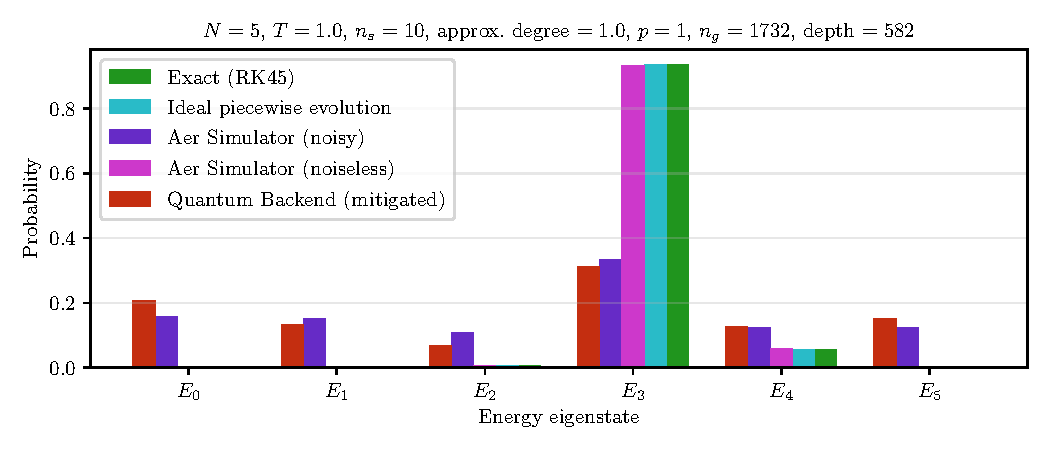
\includegraphics{img/final_comparison_one_hot.pdf}
    \caption{Quantum state driving of LMG $N=5$ model in one-hot encoding along path defined in Eq. \eqref{eq:driving_path}.}
    \label{fig:final_comparison_one_hot}
\end{figure}
\begin{figure}[h]
    \centering
    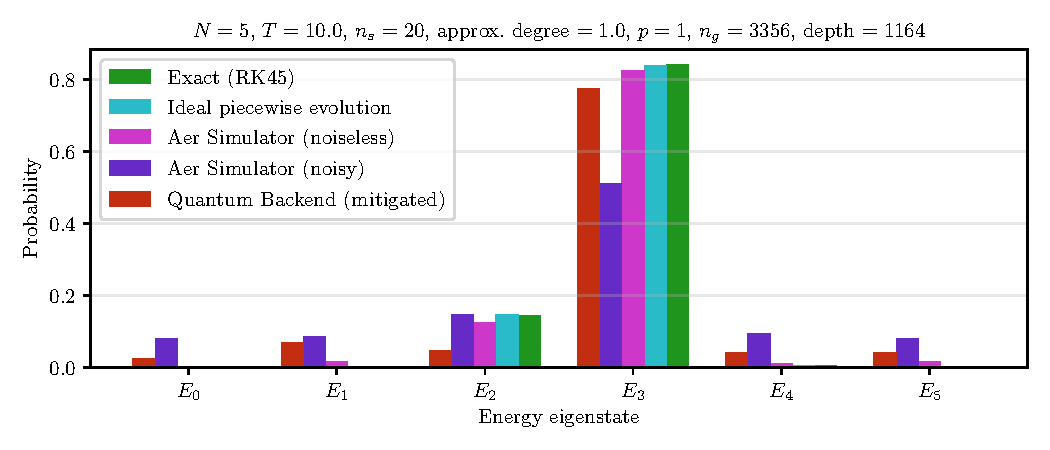
\includegraphics{img/final_comparison_one_hot_T=10.pdf}
    \caption{Quantum state driving of LMG $N=5$ model in one-hot encoding along path defined in Eq. \eqref{eq:driving_path} for longer driving time.}
    \label{fig:final_comparison_one_hot_T=10}
\end{figure}

\subsection{Discussion: One-hot vs Binary Encoding Performance}

\section{Problem Statement}
Empirical results show a counter-intuitive crossover in encoding performance:
\begin{itemize}
    \item \textbf{Short Time ($T=1, n_s=10$):} One-hot encoding performs significantly \textit{worse} than binary.
    \item \textbf{Long Time ($T=10, n_s=20$):} One-hot encoding performs \textit{better}, leveraging lower circuit depth.
\end{itemize}
This note summarizes the physical error channels and complexity factors driving this behavior.



\section{Explaining the discrepancy between precisions}
\brown{GPT explained, makes sense but unable to check exactly.}

At low circuit depths, gate errors are minimal. Performance is dominated by the cost of the encoding, where one-hot is at a severe disadvantage. Also it uses more qubits so the readout error plays a bigger role.

\subsection{Qubit Overhead and Readout Fidelity}
\begin{itemize}
    \item \textbf{System Size:} One-hot requires $N+1=6$ qubits vs. Binary $\lceil \log_2(6) \rceil = 3$ qubits.
    \item \textbf{Scaling Penalty:} Successful readout probability scales as $(1-\epsilon)^n$. With $\epsilon \approx 2\%$, one-hot suffers a $\sim 6\%$ lower fidelity floor purely due to simultaneous measurement of extra qubits.
    \item \textbf{Idle Decay ($T_1$):} The probability of a random $T_1$ decay event scales linearly with qubit count, making the 6-qubit register twice as susceptible to amplitude damping during idle times.
\end{itemize}

\subsection{Leakage and Subspace Orthogonality}
One-hot encoding is exceptionally sensitive to amplitude damping ($T_1$) due to its sparse subspace.
\begin{itemize}
    \item \textbf{One-Hot:} Logical states have Hamming weight $1$ (e.g., $\ket{001000}$). A single decay $1 \to 0$ maps the state to the vacuum $\ket{000000}$. This state is orthogonal to the logical subspace, contributing zero to the energy expectation $\braket{E}$ and manifesting as massive signal loss.
    \item \textbf{Binary:} Utilizes 75\% of the Hilbert space ($6/8$ states). A decay event (e.g., $\ket{111} \to \ket{011}$) often maps to another valid physical state, resulting in a smaller error contribution compared to total leakage.
\end{itemize}

\subsection{Measurement Complexity (Primary Issue)}
Projectors onto energy eigenstates $\hat{P}_k = \ket{E_k}\bra{E_k}$ differ drastically in complexity :
\begin{enumerate}
    \item \textbf{Pauli Weight:} One-hot projectors involve weight-6 Pauli strings (vs. weight-3 for binary), increasing individual measurement error.
    \item \textbf{Term Count:} One-hot requires summing $\sim 500$ Pauli terms vs. $\sim 36$ for binary. Statistical uncertainty scales as $\sqrt{N_{\text{terms}}}$, increasing the estimation error ratio by $\sim 3.7\times$.
\end{enumerate}

\subsection{Root Cause Analysis: Long Time Regime ($T=10$)}
For longer simulations, accumulated gate errors become the dominant noise source, favoring the one-hot encoding's efficiency.

\begin{itemize}
    \item \textbf{Circuit Depth:} Standard Trotterization in binary requires long CNOT chains for $Z\otimes Z$ terms. One-hot utilizes efficient constant-depth $XX+YY$ interactions.
    \item \textbf{Gate Count:} 
    \begin{itemize}
        \item \textbf{Binary:} $\sim 440$ CX gates, Depth $\sim 873$.
        \item \textbf{One-hot:} $\sim 195$ CX gates, Depth $\sim 361$.
    \end{itemize}
    \item \textbf{Conclusion:} At $T=10$, the substantial reduction in gate count and depth outweighs the fixed penalties from measurement complexity and qubit overhead.
\end{itemize}

\subsection{Correction Strategy}
To remediate one-hot performance at $T=1$, \textbf{Measurement Error Mitigation (Post-Selection)} is required.
\begin{itemize}
    \item \textbf{Procedure:} discard all shots where the measured bitstring Hamming weight is not exactly 1 (removing vacuum $\ket{0}^{\otimes 6}$ and multi-excitation states).
    \item \textbf{Correction:} Corrects the "Leakage" artifact described above.
\end{itemize}

\bibliography{references}

\end{document}